%==================================================================
% BAB 4 — HASIL DAN PEMBAHASAN
%
% STRUKTUR WAJIB: hasil disajikan PER RUMUSAN MASALAH, dengan urutan
% dan penomoran yang sama seperti pada matriks keterkaitan di Bab 3.
% Jangan menyajikan hasil yang tidak pernah ditanyakan.
%==================================================================

\chapter{HASIL DAN PEMBAHASAN}

\section{Gambaran Umum Responden}
Kuesioner disebarkan kepada mahasiswa aktif yang memenuhi kriteria inklusi dan
memperoleh 96 tanggapan yang lengkap. Sebaran responden berdasarkan angkatan
dan frekuensi penggunaan sistem disajikan pada \cref{tab:responden}.

\begin{table}[H]
    \centering
    \caption{Karakteristik responden}
    \label{tab:responden}
    \begin{tabular}{|l|c|c|}
        \hline
        \textbf{Karakteristik} & \textbf{Jumlah} & \textbf{Persentase} \\ \hline
        Angkatan 2022 & 31 & 32,3\% \\ \hline
        Angkatan 2023 & 34 & 35,4\% \\ \hline
        Angkatan 2024 & 31 & 32,3\% \\ \hline
        \textbf{Total} & \textbf{96} & \textbf{100\%} \\ \hline
    \end{tabular}
\end{table}

\section{Hasil Pengujian Instrumen}
Seluruh 22 butir dinyatakan valid karena nilai $r_{hitung}$ berada di atas
$r_{tabel}$ sebesar 0,201 pada taraf signifikansi 5\%. Nilai
\textit{Cronbach's alpha} sebesar 0,912 menunjukkan instrumen reliabel untuk
digunakan pada data penelitian ini.

% ==================================================================
% HASIL — disusun per rumusan masalah
% Perhatikan \label pada setiap subbab: label inilah yang dirujuk
% oleh matriks keterkaitan di Bab 3.
% ==================================================================

\section{Tingkat Kualitas Layanan}
\label{sec:hasil-rq1}
% Menjawab RQ1

Hasil pengukuran tingkat kinerja pada ketiga dimensi WebQual 4.0 disajikan pada
\cref{tab:dimensi}.

\begin{table}[H]
    \centering
    \caption{Tingkat kinerja per dimensi}
    \label{tab:dimensi}
    \begin{tabular}{|l|c|c|c|}
        \hline
        \textbf{Dimensi} & \textbf{Jumlah butir} & \textbf{Rata-rata} & \textbf{Kategori} \\ \hline
        \textit{Usability}                  & 8 & 3,12 & Cukup \\ \hline
        \textit{Information quality}        & 7 & 3,68 & Baik  \\ \hline
        \textit{Service interaction quality}& 7 & 3,54 & Baik  \\ \hline
    \end{tabular}
\end{table}

Berdasarkan \cref{tab:dimensi}, dimensi \textit{usability} memperoleh nilai
rata-rata terendah, yaitu 3,12, sedangkan \textit{information quality}
memperoleh nilai tertinggi sebesar 3,68.

\section{Kesenjangan Kepentingan dan Kinerja}
\label{sec:hasil-rq2}
% Menjawab RQ2

Perbandingan tingkat kepentingan dan tingkat kinerja pada setiap dimensi
disajikan pada \cref{tab:gap}.

\begin{table}[H]
    \centering
    \caption{Kesenjangan kepentingan dan kinerja per dimensi}
    \label{tab:gap}
    \begin{tabular}{|l|c|c|c|}
        \hline
        \textbf{Dimensi} & \textbf{Kepentingan} & \textbf{Kinerja} & \textbf{Kesenjangan} \\ \hline
        \textit{Usability}                  & 4,41 & 3,12 & $-1{,}29$ \\ \hline
        \textit{Information quality}        & 4,22 & 3,68 & $-0{,}54$ \\ \hline
        \textit{Service interaction quality}& 4,05 & 3,54 & $-0{,}51$ \\ \hline
    \end{tabular}
\end{table}

Seluruh dimensi memperoleh nilai kesenjangan negatif, yang menunjukkan kinerja
belum memenuhi harapan pengguna. Kesenjangan terbesar terjadi pada dimensi
\textit{usability}, khususnya pada butir kemudahan navigasi sebesar $-1{,}58$.

\section{Prioritas Perbaikan}
\label{sec:hasil-rq3}
% Menjawab RQ3

Pemetaan seluruh butir ke dalam diagram kartesius IPA ditunjukkan pada
\cref{fig:kuadran}.

\begin{figure}[H]
    \centering
    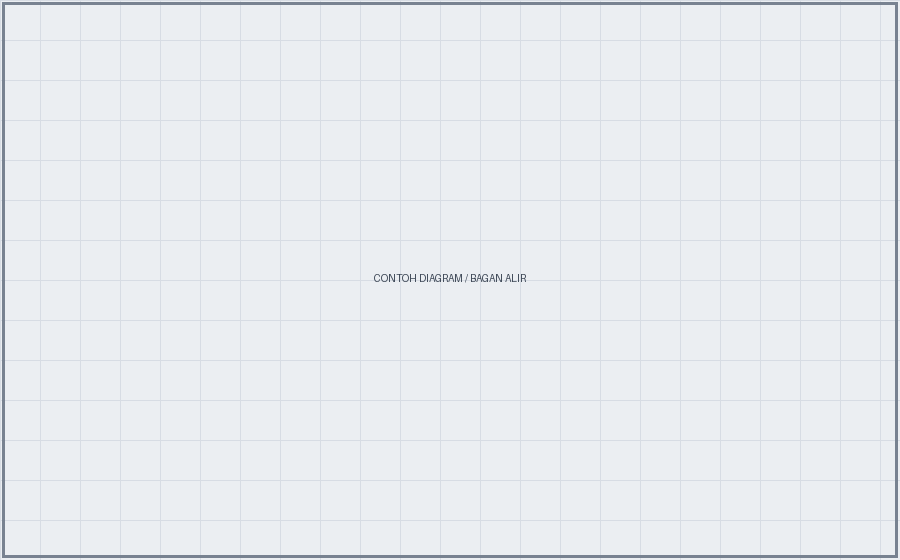
\includegraphics[width=0.7\linewidth]{contoh-diagram}
    \caption{Pemetaan kuadran \textit{Importance-Performance Analysis}}
    \label{fig:kuadran}
\end{figure}

Sebanyak lima butir berada pada kuadran prioritas utama, yaitu kuadran dengan
tingkat kepentingan tinggi namun tingkat kinerja rendah. Kelima butir tersebut
disajikan pada \cref{tab:prioritas}.

\begin{table}[H]
    \centering
    \caption{Butir pada kuadran prioritas utama}
    \label{tab:prioritas}
    \footnotesize
    \begin{tabular}{|c|p{7.5cm}|c|c|}
        \hline
        \textbf{No} & \textbf{Butir} & \textbf{Kepentingan} & \textbf{Kinerja} \\ \hline
        1 & Kemudahan menemukan menu yang dibutuhkan & 4,58 & 3,00 \\ \hline
        2 & Kejelasan alur pengisian rencana studi   & 4,52 & 3,05 \\ \hline
        3 & Kemudahan mempelajari cara pengoperasian & 4,44 & 3,10 \\ \hline
        4 & Kejelasan pesan kesalahan sistem         & 4,39 & 3,08 \\ \hline
        5 & Kemudahan navigasi antarhalaman          & 4,61 & 3,03 \\ \hline
    \end{tabular}
\end{table}

Kelima butir tersebut seluruhnya berasal dari dimensi \textit{usability} dan
berkaitan dengan navigasi serta kejelasan alur, bukan dengan ketersediaan
fitur.

% ==================================================================
% PEMBAHASAN — juga disusun per rumusan masalah
%
% POLA EMPAT LANGKAH untuk setiap subbab pembahasan:
%   (1) nyatakan ulang temuan secara ringkas;
%   (2) bandingkan dengan penelitian terdahulu YANG SAMA dengan yang
%       diperkenalkan pada latar belakang Bab 1;
%   (3) jelaskan mengapa sejalan atau mengapa berbeda;
%   (4) tarik implikasinya.
%
% Perhatikan bahwa pembahasan di bawah memuat KEDUANYA: temuan yang
% sejalan DAN temuan yang bertentangan dengan penelitian terdahulu.
% Temuan yang bertentangan bukan kelemahan, melainkan bahan analisis.
% ==================================================================

\section{Pembahasan}

\subsection{Pembahasan Tingkat Kualitas Layanan}
% Membahas hasil pada Subbab \ref{sec:hasil-rq1}

Hasil pada Subbab \ref{sec:hasil-rq1} menunjukkan dimensi \textit{usability}
memperoleh skor kinerja terendah di antara ketiga dimensi. Temuan ini sejalan
dengan hasil \citet{wijaya2022}, yang juga menemukan \textit{usability} sebagai
dimensi dengan penilaian terendah pada sistem informasi akademik, dengan
keluhan navigasi sebagai penyumbang utama.

Kesesuaian ini menguatkan dugaan bahwa persoalan utama sistem informasi
akademik terletak pada arsitektur informasi antarmuka, bukan pada kelengkapan
fitur maupun keakuratan data yang disajikan. Implikasinya, upaya perbaikan yang
menambah fitur baru berpotensi tidak menyelesaikan keluhan pengguna selama
persoalan navigasi belum dibenahi.

\subsection{Pembahasan Kesenjangan Kepentingan dan Kinerja}
% Membahas hasil pada Subbab \ref{sec:hasil-rq2}

Hasil pada Subbab \ref{sec:hasil-rq2} menunjukkan seluruh dimensi memiliki
kesenjangan negatif, dengan kesenjangan terbesar pada \textit{usability}.
Temuan ini berbeda dengan \citet{pratama2023} yang melaporkan
\textit{service interaction quality} sebagai dimensi paling berpengaruh
terhadap kepuasan pengguna.

Perbedaan tersebut dapat dijelaskan melalui karakteristik pengguna. Responden
pada penelitian \citet{pratama2023} merupakan pengguna insidental layanan
pemerintah daerah yang berinteraksi langsung dengan petugas, sehingga aspek
interaksi layanan menjadi menonjol. Sebaliknya, responden pada penelitian ini
menggunakan sistem secara mandiri tanpa pendampingan petugas, sehingga
kemudahan penggunaan antarmuka menjadi aspek yang paling dirasakan. Penjelasan
ini konsisten dengan \citet{sari2024} yang menyatakan hasil pengukuran kualitas
layanan sangat dipengaruhi karakteristik pengguna dan pola penggunaannya.

\subsection{Pembahasan Prioritas Perbaikan}
% Membahas hasil pada Subbab \ref{sec:hasil-rq3}

Hasil pada Subbab \ref{sec:hasil-rq3} menempatkan lima butir pada kuadran
prioritas utama, seluruhnya berkaitan dengan navigasi dan kejelasan alur.
Penelitian terdahulu yang menggunakan WebQual 4.0 umumnya berhenti pada
penyajian skor per dimensi \citep{wijaya2022, pratama2023}, sehingga belum
menghasilkan urutan prioritas pada tingkat butir.

Pemetaan kuadran pada penelitian ini menunjukkan bahwa meskipun dimensi
\textit{information quality} memperoleh skor tertinggi, terdapat butir di
dalamnya yang tetap masuk kuadran prioritas rendah karena tingkat
kepentingannya juga rendah. Temuan ini menegaskan bahwa keputusan perbaikan
tidak dapat didasarkan pada skor dimensi semata, melainkan perlu
mempertimbangkan tingkat kepentingan tiap butir menurut pengguna.
